\documentclass{llncs}

% For FIGURES: (1) include figures and (2) float position of figures
\usepackage{graphicx}
\usepackage{subfigure,dblfloatfix} %to fix the problem of [h!] [t!] [!b]

% For TABLES: (1) columns with predefined width (2) to make colored cells
\usepackage{array} 
\newcolumntype{L}[1]{>{\raggedright\let\newline\\\arraybackslash\hspace{0pt}}m{#1}}
\newcolumntype{C}[1]{>{\centering\let\newline\\\arraybackslash\hspace{0pt}}m{#1}}
\newcolumntype{R}[1]{>{\raggedleft\let\newline\\\arraybackslash\hspace{0pt}}m{#1}}
\usepackage[]{colortbl}

\usepackage{bbding}
\usepackage{pifont}
\usepackage{wasysym}
\usepackage{amssymb}

\begin{document}

\title{\huge DDoS Filtering Tool\\ \small A Design Paper}

\author{Jos\'e Jair Santanna \and Julik Keijer}
\institute{University of Twente, the Netherlands\\
\email{j.j.santanna@utwente.nl,keijerjs@gmail.com}\\ 
\texttt{http://ddosdb.org/ddosfiltering}}
\maketitle             

%\begin{abstract}
%\end{abstract}

\section{Introduction}
Process a large volume of data ``at home''.

\section{Collaborators Requirement}

\noindent
\textsc{Main requirements:} 
\begin{itemize}
	\item Facilitate the removal of any private information that can be potentially used for identifying either the collaborators or their clients;
	\item Generate a summary information of source IP addresses that were potentially involved in the attack;
	\item Use the summary information of source IP addresses to classify the attack type;
	\item Generate a summary of the attack; 
	\item Generate a new network file with only the filtered IP addresses attack records.
\end{itemize}

\noindent
\textsc{Additional requirements:}
\begin{itemize}
	\item Process the traffic at the collaborators' infrastructure to avoid leak of information;
	\item Facilitated the deployment of the filtering tool; 
	\item Speedup the loading process of visualizations;
	\item Create simple and meaningful visualizations;
	\item Have a dynamic (and manual) filtering interface;
	\item Highlight outliers.
\end{itemize}

\section{Tasks \& Design Decisions}

The achieve the majority of the requirements of collaborators we identify the following tasks:
\begin{enumerate}
	\item Receive an uploaded network file that contains a DDoS attack (pcap[ng] or nfdump types);	
	\item Pre-filter the uploaded network file keeping only the ingress traffic;
	\item Highlight the potential attack targets, i.e., the destination IP addresses that received more network traffic);
	\item Highlight the IP protocol that generates more network traffic towards the highlighted destination IP address;
	\item Present summarized information of source IPs that sent traffic using the highlighted IP protocol;
	\item Highlight (and manually remove) the source IPs that does not follow an attack pattern (outliers);
	\item Classify the set of remaining source IPs as a type of DDoS attack;
	\item[*8.] Use the set of remaining source IPs to filter the pre-filtered traffic (output of step 2) towards identify multi-vector attacks;  
	\item[9.] Repeat steps 3, 4, 5 and 6 until the collaborator is satisfied about the remaining information;
	\item[10.] Generate a new network attack file with only the remaining information;
	\item[11.] Export the new network attack file and the summary of the attack to DDoSDB.
\end{enumerate}

We decided to split the tasks in five main modules, depicted in Fig~\ref{fig:modules}: (i) \textsf{input}, (ii) \textsf{processing}, (iii) \textsf{visualization}, (iv) \textsf{classification}, and (v) \textsf{output}. Additionally, we include an extra module named \textsf{conversion} to optimize the \textsf{processing module}. Each module is detailed in the further subsections.

\begin{figure}[!ht] 
\centering 
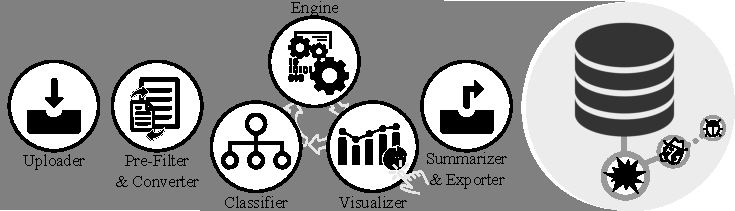
\includegraphics[]{figs/framework.pdf}
\caption{DDoS filtering tool modules.} 
\label{fig:modules} 
\end{figure}

\subsection{Input Module}
%objective
\subsubsection{Requirements}
\subsubsection{Design decisions}

\subsection{Conversion \& Prefiltering Module}
%objective: filter the input file and keep only required fields
\subsubsection{Requirements}
\subsubsection{Design decisions}
\begin{table}[h!] 
\small 
\center 
\caption{Attack information shared by initiative.}
\label{tab:attack_fields} 

\begin{tabular}{|c| l | c |c|c|c|c|c|} 
\hline
&\textbf{Information}      & \textbf{Obtained}&\cite{digitalattackmap2013web} &
\cite{norse2015web}& \cite{ipew2015web}  & \cite{fireeye2015web} &
\cite{kaspersky2015web2}\\ \hline

1&Start time 	&field&  $\checkmark$	& $\checkmark$	& ~& ~ & ~    \\ \hline    
2&Duration 		&field*& $\checkmark$	& ~ & ~& ~ & ~   \\ \hline 
3& Bit rate (peak)	&field*& $\checkmark$	& ~ & ~ & ~ & ~\\ \hline 
4& Packet rate (peak) & field*&&&&&\\ \hline
5&\# Src. IPs &field*&&&&&\\\hline	
6&\# restricted Src. IPs & enrich &&&&&\\\hline 
7&\# Src. IPs with fragm. & field&&&&& \\\hline
8&Src.  port (interval)	&field& $\checkmark$	& ~ & ~ & ~ & ~   \\\hline 
9&Dst.  port (interval) &field& $\checkmark$	& $\checkmark$	& ~ & ~ & $\checkmark$\\ \hline 
10&Attack type&heuristic& $\checkmark$ & $\checkmark$	& $\checkmark$ &~ & $\checkmark$    \\ \hline 
11&+Spoofed attack type?&heuristic& &&&&\\ \hline 
12&+Fragmented attack type?&heuristic& &&&&\\ \hline 
13&+Reflected attack type?&heuristic& &&&&\\ \hline 
14&Attack responsible (blame)& manual&&&&&\\\hline\hline\hline

\rowcolor{red}15&Dst.  IP &field& ~ & ~ & $\checkmark$& ~ & ~ \\\hline
16&Dst. IP country&enrich& $\checkmark$ & $\checkmark$	& $\checkmark$& $\checkmark$ & ~ \\ \hline 
\rowcolor{red}17&Dst. IP City &enrich& ~ & $\checkmark$	& ~ & ~ & ~   \\\hline 
\rowcolor{red}18&Dst. IP ASN &enrich& ~ & $\checkmark$ & ~ & ~ & ~ \\ \hline\hline\hline

19&Src.  IP &field& ~ &$\checkmark$ & $\checkmark$& ~ & ~    \\ \hline 
20&Src. IP country	&enrich&$\checkmark$ & $\checkmark$ & $\checkmark$& $\checkmark$ & $\checkmark$   \\
\hline    
21&Src.  IP city &enrich& ~ & $\checkmark$	& ~ & ~ & ~   \\  \hline
22&Src. IP ASN &enrich& ~ & $\checkmark$	& ~ & ~ & ~ \\ \hline 
23&Src. IP \# total packets&field&&&&&\\ \hline
24&Src. IP \# frag. packets  &field&&&&&\\ \hline 
25&Src. IP data rate & field*&&&&&\\ \hline
26&Src. IP packet rate & field* &&&&&\\ \hline
27&Src. IP restricted?  &enrich&&&&& \\ \hline 
28&Src. IP packet length &field &&&&&\\ \hline 
29&Src. IP TTL  &field &&&&&\\ \hline
\rowcolor{yellow}30&Src. IP TCP flags &field &&&&&\\ \hline 
\rowcolor{yellow}31&Src. IP HTTP payload* & field&&&&&\\ \hline
\rowcolor{yellow}32&Src. IP DNS query  & field&&&&&\\ \hline 
\rowcolor{yellow}33&Src. IP open ports &enrich&&&&&\\ \hline 

\end{tabular} 
\end{table}


\subsection{Processing and Visualization Module}
%objective
\subsubsection{Requirements}
\subsubsection{Design decisions}

\subsection{Classification Module}
%objective
\subsubsection{Requirements}
\subsubsection{Design decisions}

\subsection{Output Module}
%objective
\subsubsection{Requirements}
\subsubsection{Design decisions}






Web-based that performs offline filtering;




\section{Preliminary results}
\end{document}
